\documentclass[a4paper]{article}

\usepackage{graphicx}
\usepackage{amsmath,amssymb}
\usepackage{hyperref}
\usepackage{multirow}
\usepackage{float}

\title{Sprechen}
\author{}
\date{}

\begin{document}
    \maketitle
    
    Wie läuft die Prüfung ab?
    
    Die mündliche Prüfung wird stets von zwei lizenzierten Prüfern bzw.\ Prüferinnen durchgeführt und besteht aus drei Teilen. Sie kann entweder als Einzelprüfung mit einem Teilnehmer bzw.\ einer Teilnehmerin oder als Paarprüfung mit zwei Teilnehmenden stattfinden. Das Prüfungsgespräch dauert bei der Paarprüfung circa 16 Minuten, bei einer Einzelprüfung etwas weniger.
    
    Während der Prüfung sollen interessante Gespräche entstehen, in denen beide Prüfungsteilnehmer bzw.\ Teilnehmerinnen möglichst zu gleichen Teilen zu Wort kommen. Aufgabe der Teilnehmer und Teilnehmerinnen ist es, möglichst ausführlich auf Fragen zu antworten und auf die Beiträge des Partners oder der Partnerin (Paarprüfung) bzw.\ die Beiträge des Prüfers oder der Prüferin (Einzelprüfung) einzugehen.
    
    
    \section{Teil 1}
        Über sich sprechen (ca.\ 2 Minuten pro Teilnehmer bzw.\ Teilnehmerin)
        
        Beide Teilnehmer bzw.\ Teilnehmerinnen erhalten das gleiche Aufgabenblatt. Sie stellen sich nacheinander anhand der Stichpunkte auf dem Arbeitsblatt vor. Beiden wird außerdem eine Zusatzfrage von einem Prüfer bzw.\ einer Prüferin gestellt.
        
        \begin{figure}[H]
            \centering
            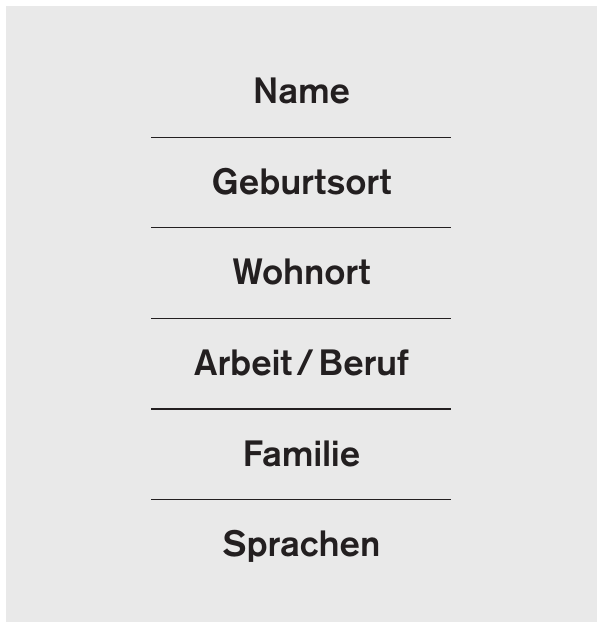
\includegraphics[width=0.9\textwidth]{teil_1_teilen.png}
        \end{figure}
    
    
    \section{Teil 2}
        Über Erfahrungen sprechen (ca.\ 3 Minuten pro Teilnehmer bzw.\ Teilnehmerin)
        
        Beide Teilnehmer bzw.\ Teilnehmerinnen erhalten ein Bild zu einem Thema. Die Bilder sind unterschiedlich. Die Teilnehmer bzw.\ Teilnehmerinnen sprechen nacheinander über ihr Bild. Jeweils im Anschluss stellt der Prüfer bzw.\ die Prüferin zusätzliche Fragen, gibt Sprechimpulse oder Prompts, in denen er bzw.\ sie das Gesagte aufgreifen kann. Die Teilnehmer und Teilnehmerinnen können sich auch untereinander über ihre Erfahrungen austauschen, werden dazu aber nicht aufgefordert.
        
        \textbf{English}
        
        Talking about experiences (approx.\ 3 minutes per participant). Both participants receive a picture on a topic. The pictures are different. The participants speak one after another about their picture. Afterwards, the examiner asks additional questions, gives speaking prompts, or prompts in which he or she can pick up on what was said. The participants can also exchange views about their experiences with each other, but they are not prompted to do so.
        
        \begin{figure}[H]
            \centering
            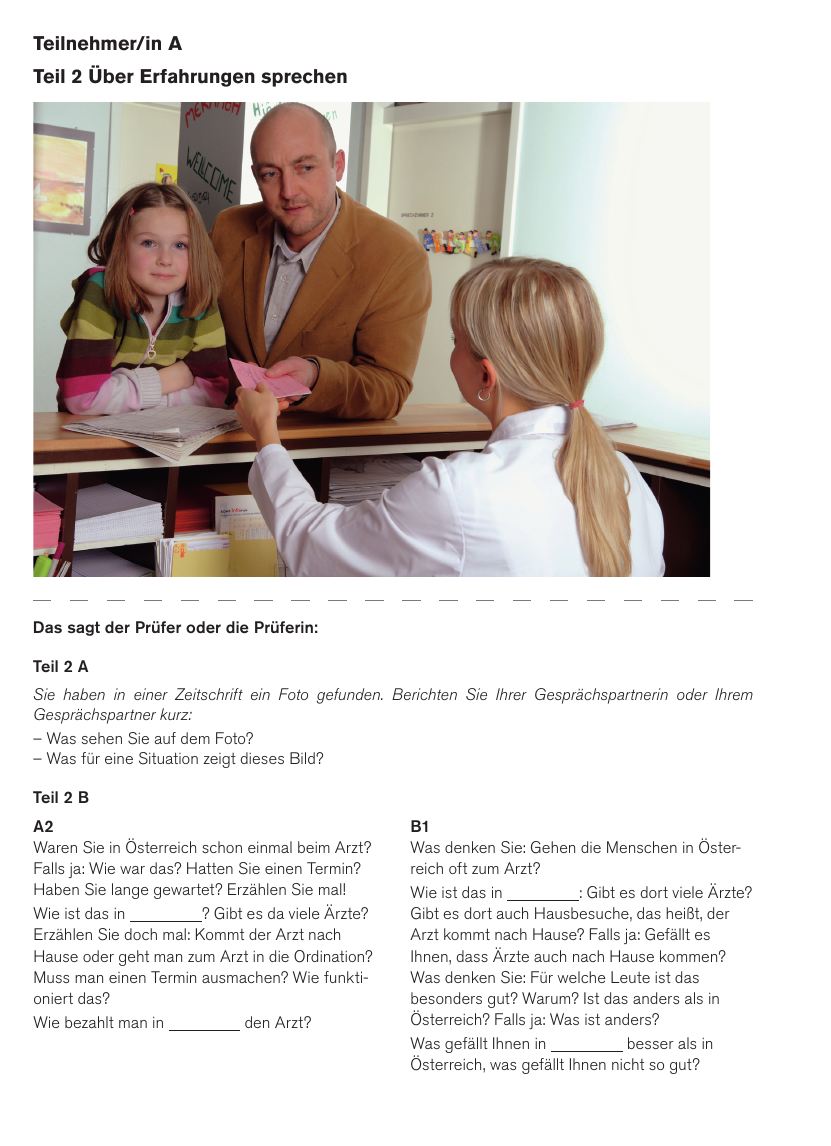
\includegraphics[width=0.9\textwidth]{teil_2_a_beispiel.png}
        \end{figure}
        
        \begin{figure}[H]
            \centering
            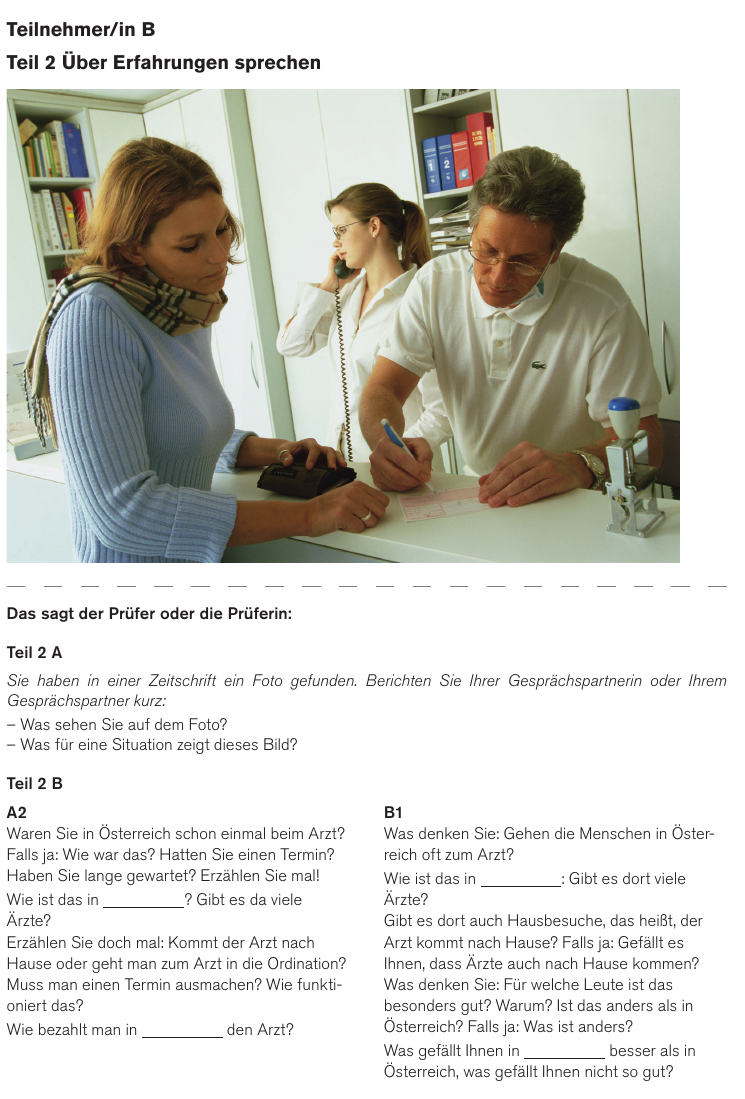
\includegraphics[width=0.9\textwidth]{teil_2_b_beispiel.png}
        \end{figure}
    
    
    \section{Teil 3}
        
        \subsection{A}
            Gemeinsam etwas planen (ca.\ 6 Minuten für beide Teilnehmer bzw.\ Teilnehmerinnen)
            
            Beide Teilnehmer bzw.\ Teilnehmerinnen erhalten das gleiche Aufgabenblatt. Ihre Aufgabe besteht darin, gemeinsam etwas zu planen. Dazu sollen sie sich ihre Ideen mitteilen, Vorschläge machen und auf die Vorschläge des Partners oder der Partnerin reagieren. Die Stichpunkte auf dem Arbeitsblatt helfen dabei.
            
            \textbf{English}
            
            Plan something together (about 6 minutes for both participants). Both participants receive the same task sheet. Their task is to plan something together. To do this, they should communicate their ideas, make suggestions, and respond to the suggestions of their partner. The bullet points on the worksheet help with this.
            
            \begin{figure}[H]
                \centering
                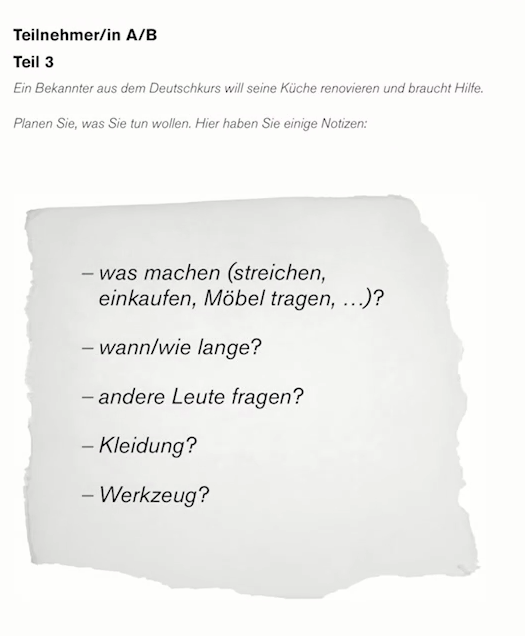
\includegraphics[width=0.9\textwidth]{teil_3_a_beispiel.png}
            \end{figure}
        
        \subsection{B}
            Das sagt der Prüfer oder die Prüferin:
            
            \medskip
            \textbf{Teil 2 A}
            
            Sie haben in einer Zeitschrift ein Foto gefunden. Berichten Sie Ihrer Gesprächspartnerin oder Ihrem Gesprächspartner kurz.
            
            \begin{itemize}
                \item Was sehen Sie auf dem Foto?
                \item Was für eine Situation zeigt dieses Bild?
            \end{itemize}
            
            \textbf{Teil 2 B}
            
            \textbf{A2}
            
            Wie ist das in \underline{\hspace{2cm}}? Gibt es da im Winter Schnee?
            
            Falls ja: Was tun die Menschen, wenn es schneit?\\
            Falls nein: Wie ist das im Winter in \underline{\hspace{2cm}}?\\
            Wie ist das Wetter? Was machen die Menschen?\\
            Machen die Menschen Sport? Erzählen Sie einmal!
            
            \medskip
            \textbf{B1}
            
            Hat es schon einmal geschneit, seit Sie in Österreich sind?\\
            Wann war das? Wie war das? Erzählen Sie mal!
            
            Fahren Sie oder Bekannte von Ihnen Ski oder Schlitten?\\
            Falls ja: Erzählen Sie mal: Wann und wo waren Sie das letzte Mal Ski oder Schlitten fahren? Wie war das?\\
            Falls nein: Würden Sie das gerne einmal ausprobieren? Was machen Sie sonst gerne im Winter?
            
            Wie ist der Winter in \underline{\hspace{2cm}}, wird es dort auch kalt und schneit es?\\
            Wie verbringen die Menschen in \underline{\hspace{2cm}} den Winter?\\
            Ist es anders als hier in Österreich?
            
            \medskip
            \textbf{English (exact translation):}
            
            The examiner says:
            
            \medskip
            \textbf{Part 2 A}
            
            You have found a photo in a magazine. Briefly tell your conversation partner about it.
            
            \begin{itemize}
                \item What do you see in the photo?
                \item What kind of situation does this picture show?
            \end{itemize}
            
            \textbf{Part 2 B}
            
            \textbf{A2}
            
            How is it in \underline{\hspace{2cm}}? Is there snow there in winter?
            
            If yes: What do people do when it snows?\\
            If no: How is winter in \underline{\hspace{2cm}}?\\
            How is the weather? What do people do?\\
            Do people do sports? Tell about it!
            
            \medskip
            \textbf{B1}
            
            Has it ever snowed since you have been in Austria?\\
            When was that? How was it? Tell about it!
            
            Do you or someone you know ski or go sledding?\\
            If yes: Tell us: When and where was the last time you went skiing or sledding? How was it?\\
            If no: Would you like to try it once? What else do you like to do in winter?
            
            How is winter in \underline{\hspace{2cm}}? Does it also get cold and snow there?\\
            How do people in \underline{\hspace{2cm}} spend the winter?\\
            Is it different from here in Austria?
            
            \begin{figure}[H]
                \centering
                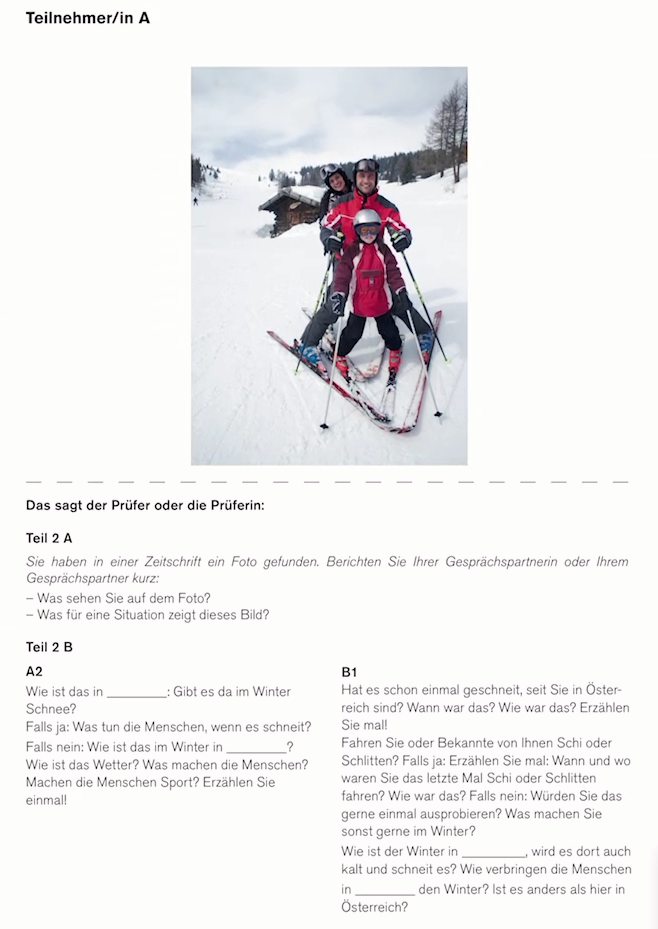
\includegraphics[width=0.9\textwidth]{teil_3_b_beispiel.png}
            \end{figure}

\end{document}